\documentclass{article}
\usepackage{inputenc}
\usepackage{setspace}
\usepackage[margin=0.75in]{geometry}
\usepackage[style=numeric]{biblatex}
\addbibresource{ref.bib}
\usepackage{float}
\usepackage{graphicx}
\graphicspath{ {./images/} }


\onehalfspace
\setlength{\parindent}{0pt}
\setlength{\parskip}{1em}



\begin{document}

\begin{center}
  \LARGE{\textbf{Real-world Functional Programming}} \\
  \Large{Project Report} \\
  \normalsize{14274056 Junsong Yang (psyjy3)} \\
  \today
\end{center}


\begin{normalsize}
  \section{Introduction}
  In this section, the general idea about this project will be introduced as
  well as how this project would fit for this module.

  The project is called recipe house, which is a recipe recommendation service
  based on the ingredients.The logic behind it is quite simple. It would require
  users to input whatever ingredients they have, then it will return recipes
  that used those ingredients. This project includes two parts: a back-end
  server and a web interface. Since I don't have any recipe database, the
  back-end server will query a third-party API for recipe info and trim the
  returned data in JSON and return the trimmed data as a response to the web
  interface.

  The third party APIs that I will use are provided by Edamam. They have over 2
  millions of recipes specified by diets, calories, nutrient ranges and simply
  just ingredients.

  This project idea was used to compete in ATOS IT Challenge and was
  shortlisted(top 20 worldwide). The back-end was written in Go as well as the
  web interface with a bit vanilla javascript, but it was not quite finished.
  Hence, this idea will be reimplemented in a different approach for this
  project.

  As for how this project may fit for 10 credits:
  \begin{itemize}
  \item[]{learning scala for backend (about 20 hrs)}
  \item[]{learning React (with any host language) (20 hrs)}
  \item[]{revisit web technologies (HTML CSS) (10 hrs)}
  \item[]{implementation of the back-end (15 hrs)}
  \item[]{implementation of the web interface (15 hrs)}
  \item[]{report writing (20 hrs)}  
  \end{itemize}

  A successful project would be a working web interface that allowed user to use
  either text-based or image based search for recipes based on what ingredients
  they have. The front-end would sent the ingredients info to the back-end
  server via REST API. Then the back-end server will query the third-party API
  for recipes and parse the returned data and sent back to the front-end as
  response. The front-end will present the response from server to the end user. 


  \section{Technical Background}
  In this section, the technological choices made for both the back end and
  front end will be discussed in detail with justification.

  For backend server, the language of choice is Scala. Scala is a multi-paradigm
  programming language compiles to java bytecode and supports both functional
  programming and imperative programming. Hence, by using scala, we can not only
  explore functional programming in depth but also leveraging the java
  ecosystem. The backend server provides service through REST apis, therefore,
  the play framework is chosen to serve thid purpose. The play framework
  supports MVC architecture by default, but this project is not designed that
  way. The project does not include database and the frontend is implemented
  separately. Hence, only controllers will be created.

  As for the frontend interface, a javascript library called React will be used.
  The reason for that choice is that, React supports functional reactive
  programming paradigm which can be used to create graphical user interface.
  Functional reactive programming is progamming paradigm that been studied over
  the years and there are a few attemps to apply functional reactive progamming
  to graphical user interface designs. React is not purely functional by nature
  as it relies on javascript as its underlying programming language. But the
  design decisions made for this library are inspired by functional reactive
  programming. Hence, React can be used to design graphical user interface using
  functional reactive progamming.
  
  \section{Implementation}
  In this section, the general architecture of this project will be introduced
  as well as some essential implementation details.

  \subsection{Architecture}
  \begin{figure}[H]
    \centeringng
    \centerline{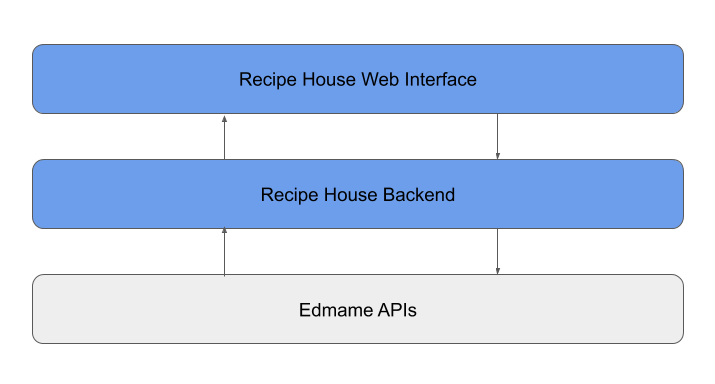
\includegraphics[scale=0.4]{archi}}
    \caption{Architecture of this project}
    \label{fig:architecture}
  \end{figure}

  Figure \ref{fig:architecture} shows the overall structure of this project.
  This project mainly consists of two parts. The recipe house web interface and
  backend server. The we interface provide an access to the end users. The name
  of ingredients can be input through the web interface. The web interface will
  requests the backend server accordingly for recipe data then those data will
  be presented to the end user through the web interface. As for the backend
  server, It provide services to the web interface through REST apis. Given the
  input from the user, the backend server will query the edamame api for recipe
  information. 

  \subsection{Backend}
  \begin{figure}[H]
    \centeringng
    \centerline{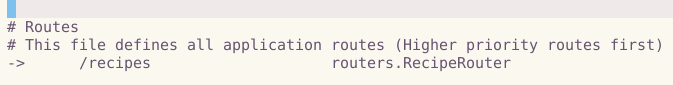
\includegraphics[scale=0.8]{route}}
    \caption{Architecture of this project}
    \label{fig:route}
  \end{figure}
  The backend server is implemented using play framework. Figure \ref{fig:route}
  shows the contains of the route file. The arrow suggested that this route is
  defined generically. Any route that matches the route defined above will be
  handled by the RecipeRouter in routers package.

  \begin{figure}[H]
    \centeringng
    \centerline{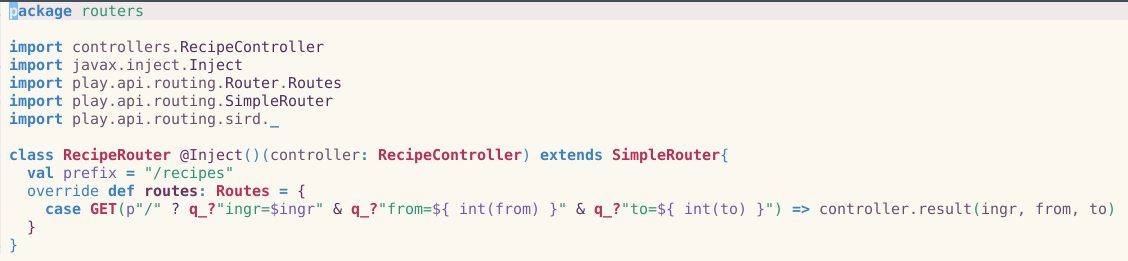
\includegraphics[scale=0.6]{router}}
    \caption{Architecture of this project}
    \label{fig:router}
  \end{figure}
  Figure \ref{fig:router} depicted the implementation of the router. The route
  here is defined using pattern matching and domain specific language provided
  by the play framework. This domain specific language will strip the parameters
  inside the url and then pass to the result function defined in the
  RecipeController. As shown in figure \ref{fig:router}, the ingr, from and to
  are passed the the result function. Specifically, the data types of those
  parameters need to be mentioned here. They are normal data types wrapped in a
  data type called Option. The Option type is equivlant to the Maybe monad in
  Haskell, it either has a value or nothing.
  

  \begin{figure}[H]
    \centeringng
    \centerline{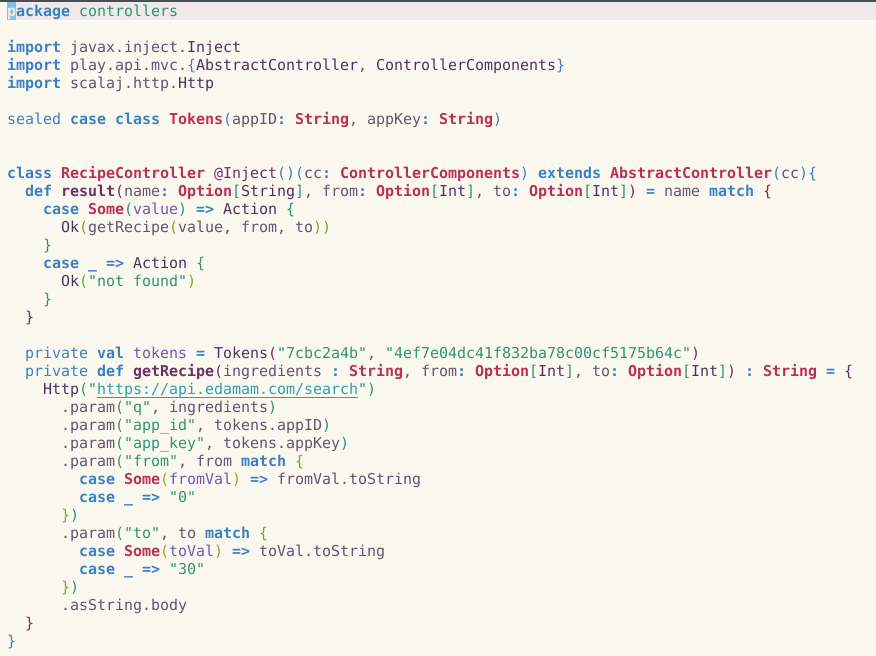
\includegraphics[scale=0.7]{controller}}
    \caption{Architecture of this project}
    \label{fig:controller}
  \end{figure}
  Figure \ref{fig:controller} shows the implementation of the RecipeController.
  This controller has two functions, the result function and the getRecipe
  function. The result function will first do the pattern matching on the name
  parameter as it contains the ingredients' name. If the name parameter contains
  some value, then the getRecipe function will be called. Otherwise, the result
  function will just return not found.

  As for the getRecipe function, it takes three parameters, ingredients, from
  and to. The from and to parameters are wrapped in Option data type as they are
  optional. The getRecipe function will query edmame api as return the response
  as the result.

  \subsection{Frontend}
  
  
  \section{Reflection}
  
\end{document}
